%  article.tex (Version 3.3, released 19 January 2008)
%  Article to demonstrate format for SPIE Proceedings
%  Special instructions are included in this file after the
%  symbol %>>>>
%  Numerous commands are commented out, but included to show how
%  to effect various options, e.g., to print page numbers, etc.
%  This LaTeX source file is composed for LaTeX2e.

%  The following commands have been added in the SPIE class 
%  file (spie.cls) and will not be understood in other classes:
%  \supit{}, \authorinfo{}, \skiplinehalf, \keywords{}
%  The bibliography style file is called spiebib.bst, 
%  which replaces the standard style unstr.bst.  

\documentclass[]{spie}  %>>> use for US letter paper
%%\documentclass[a4paper]{spie}  %>>> use this instead for A4 paper
%%\documentclass[nocompress]{spie}  %>>> to avoid compression of citations
%% \addtolength{\voffset}{9mm}   %>>> moves text field down
%% \renewcommand{\baselinestretch}{1.65}   %>>> 1.65 for double spacing, 1.25 for 1.5 spacing 
%  The following command loads a graphics package to include images 
%  in the document. It may be necessary to specify a DVI driver option,
%  e.g., [dvips], but that may be inappropriate for some LaTeX 
%  installations. 
\usepackage[]{graphicx}
\usepackage{amssymb}
\graphicspath{{pics/}}

\title{A Framework for Automatic Tuning of System Parameters and Its Use in Image Registration}

%>>>> The author is responsible for formatting the 
%  author list and their institutions.  Use  \skiplinehalf 
%  to separate author list from addresses and between each address.
%  The correspondence between each author and his/her address
%  can be indicated with a superscript in italics, 
%  which is easily obtained with \supit{}.

\author{Ren Hui Gong\supit{a} and Ziv Yaniv\supit{a}
\skiplinehalf
\supit{a}Sheikh Zayed Institute for Pediatric Surgical Innovation, Children's National Medical Center, Washington, DC 20010, USA
}

%>>>> Further information about the authors, other than their 
%  institution and addresses, should be included as a footnote, 
%  which is facilitated by the \authorinfo{} command.

%\authorinfo{Further author information: (Send correspondence to A.A.A.)\\A.A.A.: E-mail: aaa@tbk2.edu, Telephone: 1 505 123 1234\\  B.B.A.: E-mail: bba@cmp.com, Telephone: +33 (0)1 98 76 54 32}
%%>>>> when using amstex, you need to use @@ instead of @
 

%%%%%%%%%%%%%%%%%%%%%%%%%%%%%%%%%%%%%%%%%%%%%%%%%%%%%%%%%%%%% 
%>>>> uncomment following for page numbers
% \pagestyle{plain}    
%>>>> uncomment following to start page numbering at 301 
%\setcounter{page}{301} 
 
\begin{document} 
\maketitle 

%%%%%%%%%%%%%%%%%%%%%%%%%%%%%%%%%%%%%%%%%%%%%%%%%%%%%%%%%%%%% 
\begin{abstract}
The setting of system or internal parameters has significant impact on the overall performance of a system. Traditionally, such parameters are most often obtained empirically, through trial-and-error, if intrinsic knowledge about the parameters is not available. In this paper, we present a more \emph{intuitive} and \emph{systematic} framework for this type of problems, and use it to refine the system parameters of a common registration problem. We formulate the performance of the registration problem as a function of its system parameters, and use optimization techniques to search for an optimal setting for the parameters. The performance of the problem is evaluated as the overall final alignment for a group of registrations that use a set of training images. Each training image includes a segmentation of the anatomy of interest, and the quality of a registration is judged by comparing the overlap between the segmentations as induced by the registration. As a very large number of expensive registrations are performed during the optimization, a cluster of MPI-enabled computers are used to solve the problem collaboratively such that implementation of such an approach is practical. We evaluated the proposed method using a set of human abdominal CT images, and examined three different optimization algorithms. The results showed that, compared with the empirical values suggested in the published literature, our new technique was able to obtain improved system parameters that are tuned for particular applications. In addition, the proposed framework can be potentially extended to solve a large number of similar problems. 
\end{abstract}

%>>>> Include a list of keywords after the abstract 

%\keywords{parameters tuning, framework, meta-optimization, image registration, MPI-based computation}

%%%%%%%%%%%%%%%%%%%%%%%%%%%%%%%%%%%%%%%%%%%%%%%%%%%%%%%%%%%%%
\section{Motivation}

Nearly every computational system in medicine, software or hardware, has internal parameters, and the settings of the parameter values are critical to the system's overall performance. While there are well established methods to determine the parameter values for systems with analytical models (e.g. calibration parameters for imaging devices), empirical approaches through trial-and-error are commonly adopted for the majority of other parameters (e.g. special parameters in image registration that are involved in image pre-processing, similarity metric definition, function optimization, and so on). One main disadvantage of these approaches is that the obtained parameters may not be suitable for other cases, and we may not even know whether the obtained parameters are locally optimal or not. In clinical practice, ideal parameter values can differ greatly even for similar tasks such as registration of different bony structures. Fine-tuned parameters can potentially improve the performance of these applications.

In this paper, we propose a framework to automate the process of parameters tuning, and use it to refine several numerical parameters of a common registration problem. This approach formulates the performance of a system as a function of its internal parameters and uses optimization techniques to search for an optimal solution. The function is defined using a set of training examples for the system, thus it is a more systematic and resilient solution than empirical approaches. However, the function is not necessarily smooth in real applications, making optimization of such problems a challenging task. An additional potential challenge has to do with the computational complexity of the function evaluation, in some cases this can be prohibitive and requires the use of distributed computing.

Our approach to optimizing the system parameters can be viewed as a variant of meta-optimization~\cite{metaopt}. Meta-optimization is the use of optimization techniques to tune parameters of other optimization methods and has been previously applied in neural networks and various evolutionary algorithms~\cite{smit09:ece}. In this work, we aim to provide a general framework for problems in the medical domain and address the associated challenges.

%%%%%%%%%%%%%%%%%%%%%%%%%%%%%%%%%%%%%%%%%%%%%%%%%%%%%%%%%%%%%
\section{Method} 

\subsection{General Framework for System Parameters Tuning}\label{framework}

Most systems have \emph{internal settings} that are used to process some \emph{user-supplied input}. We generalize these two types of information with a vector of parameters $p$, and an abstract data structure $data$. Usually the internal parameters are fixed or user-configurable within a predefined range when the system is deployed, while the user data being processed during
production can have a large variability and the outcome is highly dependent on the setting of the internal parameters. In this work, we only consider parameters in $\mathbb{R}$ that can be numerically optimized, although other types of parameters may also be important to the system.

Assume that, for any given setting of the parameters and any given user data, we can find a function $f$ to evaluate the performance of the system, then the problem of parameters tuning can be solved by optimizing the function $f(p,data)$ with respect to parameters $p$, taking into account all possible variability of the user data. As it is difficult to predict the user data to be processed, we assume that a set of training data, denoted $\{data_i\}, i=1...N$, that captures the distribution of the expected inputs is available, then we propose a general framework to automatically solve this type of problems. 

Fig.~\ref{fig:spt_framework} illustrates the main components as well as the work-flow of this framework. An initial value of the parameters is provided to start the optimization process. In each optimization iteration, the parameters are fed into a set of $N$ instances of the system, each processes one training data set and is rated under the current setting of the parameters. The individual ratings are then collected and aggregated by a score combiner, which is in turn fed into the optimizer to produce an improved setting of the parameters.

In practice, the computation cost of this framework can be very expensive. This is mainly because the function between the parameters and the system's overall performance is usually highly non-linear and very noisy, requiring the use of population-based algorithms which are more appropriate for these type of functions. In addition, a large $N$ may be needed to represent the distribution of the user data, and each single evaluation of the system can have a high computational complexity too. To overcome these issues, we propose to implement the framework on a cluster of workstations that are connected using the Message Passing Interface (MPI) \cite{SkjellumAn1994b}. As illustrated in Fig.~\ref{fig:spt_framework}, the problem is solved using a master-slave computing model on a set of $M$ computers. The function evaluation for each training data set is evaluated in a separate slave process, and the master process is responsible for combining the individual ratings and performing the optimization. Each participating computer can simultaneously run a number of slave processes that are specified by the user.

We propose to use population-based optimization algorithms to search for an optimal setting for the defined system parameters. We evaluate three different algorithms: Particle Swarm Optimization (PSO) \cite{Kennedy95:NN}, Covariance Matrix Adaptation Evolution Strategy (CMA-ES) \cite{Hansen06}, and an adapted Brute Force (BF) search. The first two algorithms use a number of sample points in the parameter's space to drive the search process, thus they are more robust to noise and local minima. For the brute force approach, we first evaluate the function at points of a regular grid  in the parameter's space; then, starting from the best value, a second search with the Amoeba algorithm is performed.
% we will expand this in the full paper (provide more details for each algorithm).

The type of user data and definition of the function $f$ are application specific. In the next subsection, we present how this framework fits into the context of a common medical image processing task, registration.

\subsection{Automatic Tuning of Registration Parameters}

\subsubsection{Parameters to be optimized}

Deformable 3D/3D (CT/CT) image registration is a fundamental task in medical image processing. It is commonly used for constructing anatomical atlases, and enabling image-guided interventions in soft tissue structures. The registration task is usually solved using a multi-level scheme: in the first level, the global alignment between the images is estimated using a transformation with a few degrees-of-freedom (DOFs) such as rigid, similarity or affine; in the second level, registration is locally refined with a transformation with a high number of DOFs such as B-spline Free-Form Deformations (FFD). A commonly used optimizer for this problem is Gradient-Descent (GD) due to its high efficiency. However, the setting of several parameters of GD can greatly affect the overall performance of the registration. 

We consider a typical deformable registration problem that consists of a similarity registration in the first level and a B-spline FFD registration in the second level. We use our framework to tune four critical parameters of the GD optimizer. 
In the similarity registration, three types of transformation parameters need to be determined, which are rotation in the form of a versor, translation, and isotropic scaling. As the parameters are not commensurate it is common to scale their values so that changes in all values have similar effects on the change in the optimized function value. These scaling factors have a significant effect on the registration optimization process. If not appropriately set, the optimization may be biased to a subset of the transformation parameters, which yields premature termination or higher failure rate. 
In the B-spline FFD registration, one important GD parameter is the relaxation factor, which determines how much or how fast to relax the step length when the current step length no longer drives the registration. Too large or too small step sizes will affect the registration performance, especially the convergence speed. 

Values for the above-mentioned parameters have been suggested in the manual and examples of the Insight Registration and Segmentation Toolkit (ITK)\cite{itk:v2.4}; however, no reasoning is given with regard to the specific value choices, and we do not know whether they are optimal in some sense.

\subsubsection{Evaluation of registration performance}

The performance of the described registration is evaluated by performing a number of registrations with a set of training images and evaluating the overall final alignment. Each training image includes a segmentation of an anatomy of interest, and the quality of the final alignment of a registration is calculated as the complement (for minimization) of the Dice Similarity Coefficient (DSC) \cite{dsc}, which computes the ratio of overlap between the fixed and registered segmentations. 

%%%%%%%%%%%%%%%%%%%%%%%%%%%%%%%%%%%%%%%%%%%%%%%%%%%%%%%%%%%%%
\section{Results}

We used 4D abdominal CT images from five patients to evaluate the proposed method. For each patient two images that correspond to the respiratory phases end-inhale and end-exhale were used, and each image had an associated segmentation of the liver that was performed by an attending interventional radiologist. 

We used the images from end-inhale to train our proposed method, and the images from end-exhale to verify the results obtained from the training. For each of the training and verification studies, ten different registrations were formed from the five images.

We used Mattes Mutual Information \cite{Mattes03:TMI} as the similarity metric in both registration levels. The similarity registrations used about $1\%$ of voxels from the liver region for metric calculation, and were executed for 150 iterations. The B-spline deformation registrations used about $3\%$ of voxels, and were executed for 50 iterations. A $7 \times 7 \times 7$ B-spline control grid over the liver region was used to model the tissue deformations.

We studied the behaviors of the proposed method using each of the three optimization algorithms described in section \ref{framework}, and used the parameters suggested in the ITK examples as a reference for comparison. 
For PSO, 25 particles were used and 30 generations were executed. It does not need an initial value of the parameters; instead, a feasible region was used to create the particles as well as to constrain the parameters during the optimization. 
For CMA-ES, the optimization started from a user-supplied initial value, 7 particles were used in each iteration, and 100 total iterations were performed. 
For adapted BF, we placed a $5 \times 5 \times 5 \times 5$ grid over the same bounding region used for the PSO and performed function evaluations at all grid points, then an additional optimization with Amoeba was performed for 50 iterations. Each of the above experiments performed about 700 total registrations, which were executed in  parallel using 10 slave processes.

We used a cluster of four computers and the MPICH2 implementation of the MPI protocol to perform the experiments. Fig.~\ref{fig:results_training} shows the overall alignments over time for the three optimization algorithms being studied, and Table~\ref{tab:results_validation} shows the final alignments when the obtained parameters were used to register the testing images.

\section{Conclusion}

In Fig.~\ref{fig:results_training}, all three studied optimization algorithms were able to improve the overall alignments at the end of optimizations for the training images, with the best result being produced by PSO.
From Table~\ref{tab:results_validation}, we observed an overall $2\%$ improvement in final alignment for PSO, and $1\%$ for adapted BF when the obtained parameters were applied to the testing images. No improvement was observed for CMA-ES, but the results were still comparable to those obtained using the ITK suggested value. 

From those preliminary results, we can conclude that the proposed method is able to produce improved system parameters, and it is more intuitive and systematic than the conventional trial-and-error approach. In addition, the use of MPI-based computation makes it possible to perform the expensive tuning tasks with a cluster of workstations.

%%%%%%%%%%%%%%%%%%%%%%%%%%%%%%%%%%%%%%%%%%%%%%%%%%%%%%%%%%%%%
%\acknowledgments     %>>>> equivalent to \section*{ACKNOWLEDGMENTS}       
% 
%This unnumbered section is used to identify those who have aided the authors in understanding or accomplishing the work presented and to acknowledge sources of funding.  

%%%%%%%%%%%%%%%%%%%%%%%%%%%%%%%%%%%%%%%%%%%%%%%%%%%%%%%%%%%%%
%%%%% References %%%%%

\bibliography{rhgong_atosp}   %>>>> bibliography data in report.bib
\bibliographystyle{spiebib}   %>>>> makes bibtex use spiebib.bst

%============================================
\begin{figure}
\begin{center}
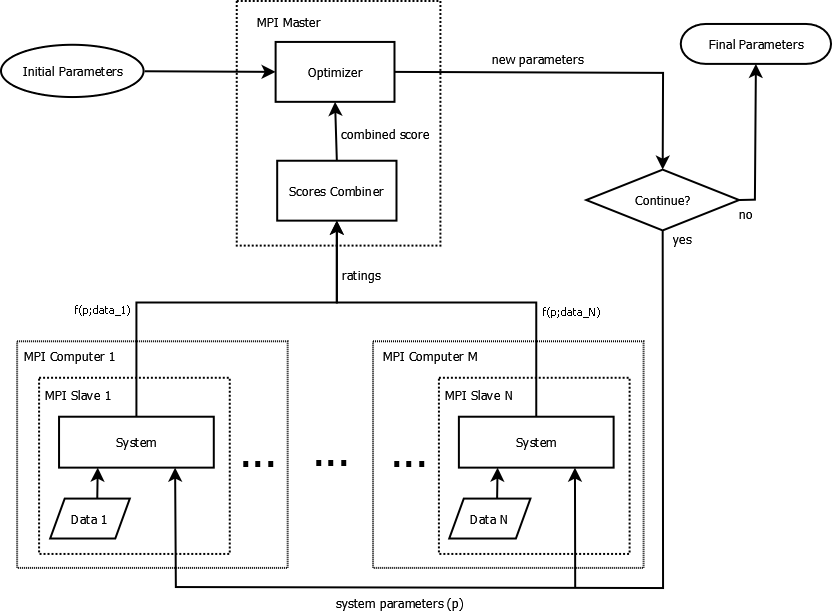
\includegraphics[width=4in]{framework}
\end{center}
\caption{General framework for system parameters tuning.}
\label{fig:spt_framework}
\end{figure}

%============================================
\begin{figure}
\begin{center}
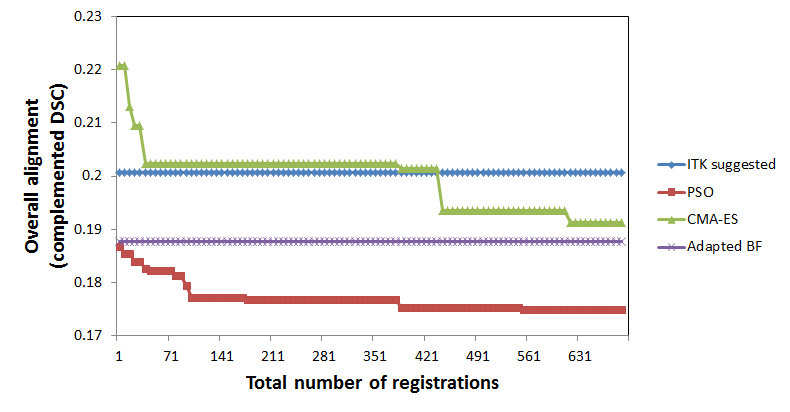
\includegraphics[width=5in]{results_training}
\end{center}
\caption{Overall alignments over time for the three optimization algorithms. The value for the adapted BF was available only at the end of the optimization. This value as well as the ITK suggested one is displayed for illustration purposes.}
\label{fig:results_training}
\end{figure}

%============================================
\begin{table}
\caption{Results with testing images: final alignments (complemented DSC) obtained from parameters suggested by ITK and our proposed method. An arrow from P\textit{A}.T\textit{X} to P\textit{B}.T\textit{Y} means registering the image of patient \textit{A} at time \textit{X} to the image of patient \textit{B} at time \textit{Y}.}
\label{tab:results_validation}
\begin{center}
%
\begin{tabular}{c|c|c|c|c}
\hline
Registration & ITK suggested & PSO & CMA-ES & Adapted BF \\
\hline \hline
P0.T50 $\rightarrow$ P1.T50 & 0.24 & 0.24 & 0.26 & 0.24 \\
\hline
P0.T50 $\rightarrow$ P2.T50 & 0.13 & 0.11 & 0.15 & 0.12 \\
\hline
P0.T50 $\rightarrow$ P3.T50 & 0.13 & 0.10 & 0.13 & 0.12 \\
\hline
P0.T50 $\rightarrow$ P4.T50 & 0.22 & 0.22 & 0.21 & 0.20 \\
\hline
P1.T50 $\rightarrow$ P2.T50 & 0.21 & 0.16 & 0.20 & 0.15 \\
\hline
P1.T50 $\rightarrow$ P3.T50 & 0.14 & 0.14 & 0.17 & 0.17 \\
\hline
P1.T50 $\rightarrow$ P4.T50 & 0.22 & 0.24 & 0.22 & 0.22 \\
\hline
P2.T50 $\rightarrow$ P3.T50 & 0.19 & 0.14 & 0.21 & 0.16 \\
\hline
P2.T50 $\rightarrow$ P4.T50 & 0.16 & 0.15 & 0.18 & 0.16 \\
\hline
P3.T50 $\rightarrow$ P4.T50 & 0.23 & 0.23 & 0.24 & 0.23 \\
\hline \hline
mean $\pm$ std.dev. & 0.19 $\pm$ 0.04 & 0.17 $\pm$ 0.05 & 0.20 $\pm$ 0.04 & 0.18 $\pm$ 0.04 \\
\hline
\end{tabular}
%
\end{center}
\end{table}

\end{document} 
